% Provenance (never printed): see sources/outline_sources.md (Year 2: monsoons; El Niño--Southern
% Oscillation; the North Atlantic Oscillation; ocean--atmosphere coupling). Definitions after the
% IPCC AR6 glossary, the NOAA CPC ENSO FAQ and NAO pages, the NWS glossary and the IMD monsoon
% FAQ; indices from the CPC data files (data/derived/bachelor-2-{oni,oni-table,roni,nino34,nao});
% figures from figdata/bachelor-2/climvar.py; values of the examples, exercises and problem
% computed in the Book 4 scratch calculator calc/ch23.py.
\chapter{Variabilidad climática}\label{ch:b2:climate-variability}

En septiembre de 2026 la superficie del mar en el Pacífico ecuatorial central promedió \qty{29.27}{\celsius},
donde el valor habitual de septiembre es de \qty{26.71}{\celsius}; más al este, partes del océano estaban
más de \qty{4}{\celsius} por encima de lo habitual, y los predictores cifraban en más de cuatro de cada cinco la
probabilidad de que el episodio superara, a finales de año, a todos los El~Niño desde 1950. Los anteriores
episodios récord, en 1982, 1997 y 2015, blanquearon y mataron corales, incendiaron bosques tropicales
y trajeron olas de calor; la captura de anchoveta del Perú cae bruscamente cuando esas aguas cálidas persisten. El
océano y la atmósfera del Pacífico tropical habían oscilado, como lo hacen cada pocos años, y la
oscilación llegó mucho más allá del Pacífico. Este
capítulo describe esas oscilaciones del clima, los monzones, El~Niño y La~Niña, la \omterm{def:b2:climate-variability:nao}{Oscilación del Atlántico
Norte}, y lo que convierte al océano en su memoria.
% ledger: data:b4-nino34, cpc:edd-2026-10, thirumalai24:bjerknes, cheung26:peru

\begin{recall}
\textbf{De los volúmenes escolares}: el tiempo y el clima; la anomalía de temperatura; la capa de mezcla,
la termoclina y el afloramiento; la retroalimentación climática. \textbf{Del volumen de primer año}: las células de
Hadley, los alisios, la zona de convergencia intertropical y su migración estacional, la circulación
de Walker, el afloramiento costero. \textbf{Del \cref{ch:b2:weather-systems}}: la corriente en chorro,
las \omterm{def:b2:weather-systems:rossby}{ondas de Rossby}, los ciclones extratropicales y el bloqueo. \textbf{De los libros de física}: la capacidad calorífica
y el primer principio de la termodinámica.
\end{recall}

\section{La variabilidad y sus medidas}\label{sec:b2:climate-variability:measures}

El tiempo cambia de un día a otro; el clima, la estadística del tiempo, también cambia, de una estación
o de un año al siguiente, incluso cuando nada exterior al sistema climático cambia. Parte de esa
variabilidad es ruido, pero buena parte se organiza en unas pocas configuraciones que se repiten, con su propia
geografía y sus propias escalas de tiempo.

\begin{definition}[Modo de variabilidad climática; índice climático; climatología]\label{def:b2:climate-variability:modes}
Un \emph{modo de variabilidad climática}\index{modo de variabilidad climatica@modo de variabilidad climática} es una configuración recurrente de
variabilidad natural del sistema climático, con su propio patrón espacial, su estacionalidad y sus escalas
de tiempo, que surge de la dinámica de la atmósfera o del acoplamiento entre el océano y la
atmósfera. Un \emph{índice climático}\index{indice climatico@índice climático} es una serie temporal construida a partir de variables
climáticas que resume el estado de esa configuración, por ejemplo la diferencia de presión al nivel del mar
entre Islandia y las Azores. La \emph{climatología}\index{climatologia@climatología} de una variable
es su media sobre un periodo de referencia, calculada para cada mes o estación del calendario; el periodo de referencia
estándar dura 30 años, actualmente 1991--2020.
\end{definition}
% ledger: ipccgl:modes, ipccgl:index, wmo:normal-30yr

Muchos modos se deben a procesos internos del sistema climático: forman parte de su
variabilidad interna. Como se repiten con sus propias escalas de tiempo, son una fuente de
predictibilidad más allá del alcance de las predicciones meteorológicas, de semanas a décadas. Los índices los hacen
medibles. Un índice se calcula a partir de anomalías, como en los volúmenes escolares, y se
suaviza.
% ledger: ipccgl:modes

\begin{method}[De las observaciones a un índice]\label{met:b2:climate-variability:index}
\begin{enumerate}
  \item Calcúlese la \omterm{def:b2:climate-variability:modes}{climatología}: la media de la variable para cada mes del calendario a lo largo del
        periodo de referencia.
  \item Réstese: la anomalía de cada mes es su valor menos la \omterm{def:b2:climate-variability:modes}{climatología} de ese mes.
        El ciclo estacional desaparece; lo que queda es la variabilidad.
  \item Suavícense las anomalías con una media móvil, la media de $n$ valores consecutivos centrada en
        cada mes, para eliminar las fluctuaciones más cortas que la configuración que interesa.
  \item Si el índice ha de compararse con otros, divídase por su desviación típica: el índice
        queda entonces estandarizado, en unidades de desviación típica.
\end{enumerate}
\end{method}

\begin{example}[Una anomalía]\label{ex:b2:climate-variability:anomaly}
La temperatura media de la superficie del mar del Pacífico ecuatorial central entre \ang{5} N y
\ang{5} S, \ang{170} W y \ang{120} W fue de \qty{29.27}{\celsius} en septiembre de 2026. Su \omterm{def:b2:climate-variability:modes}{climatología}
de septiembre es de \qty{26.71}{\celsius}, así que la anomalía fue de $29.27 - 26.71 = \qty{2.56}{\celsius}$.
En septiembre de 1997 el mismo océano estaba a \qty{28.79}{\celsius} frente a \qty{26.73}{\celsius}, una
anomalía de \qty{2.06}{\celsius}. Las dos \omterm{def:b2:climate-variability:modes}{climatologías} difieren ligeramente porque el periodo de referencia
se desplaza cada cinco años: el propio océano se ha calentado.
% ledger: data:b4-nino34, cpc:oni-def
\end{example}

\section{Los monzones}\label{sec:b2:climate-variability:monsoons}

\begin{definition}[Monzón]\label{def:b2:climate-variability:monsoon}
Un \emph{monzón}\index{monzon@monzón} es un viento de origen térmico, debido al calentamiento distinto de
una masa continental y del océano adyacente, que invierte su dirección con las estaciones, junto con
la inversión estacional de las lluvias que trae.
\end{definition}
% ledger: nws4:monsoon, ipccgl:monsoon

En tierra, el calor del Sol de verano se queda en una capa delgada cerca de la superficie, mientras que el mar mezcla
el mismo calor hacia abajo a través de su capa de mezcla, de decenas de metros de espesor, y se calienta mucho menos. El aire sobre
la tierra se calienta más, su presión en superficie baja, y el aire húmedo llega desde el mar, asciende, se enfría y
llueve; en altura el aire vuelve hacia el mar. En invierno la tierra es la superficie más fría y la circulación
se invierte. En conjunto, los monzones del planeta forman una sola configuración global que domina el ciclo
anual de las lluvias tropicales y subtropicales; su dominio se define como las regiones donde la lluvia media
del verano local supera a la del invierno en más de \qty{2.5}{mm} al día.
% ledger: nws4:monsoon, ipccgl:monsoon

\begin{omfigure}
\centering
\begin{tikzpicture}[font=\scriptsize, >=Stealth]
\foreach \col/\title in {0/{a\enspace verano}, 7.2/{b\enspace invierno}} {
  \begin{scope}[shift={(\col,0)}]
  \node[anchor=south west] at (0,3.0) {\textbf{\title}};
  \fill[ocBlue!18] (0,0) rectangle (3,0.35);
  \fill[brown!35] (3,0) -- (6.4,0) -- (6.4,0.5) -- (3,0.35) -- cycle;
  \node at (1.5,0.17) {mar};
  \node at (4.7,0.2) {tierra};
  \end{scope}
}
% summer: low over the land, inflow from the sea, rising air and rain
\node[font=\small\bfseries, ocBlue] at (0.45,0.62) {A};
\node[font=\small\bfseries, ocRed] at (4.8,0.78) {B};
\node[ocRed, anchor=west] at (5.35,0.78) {cálida};
\draw[->, thick] (1.0,0.98) -- (4.2,1.02);
\node at (2.4,0.66) {aire húmedo del mar};
\draw[->, thick] (4.8,1.15) -- (4.8,2.55);
\draw[->, thick] (4.45,2.8) -- (1.75,2.8);
\draw[->, thick] (1.4,2.6) -- (1.4,1.25);
\fill[black!15, draw=black!40] (4.0,1.9) .. controls (4.0,2.55) and (5.6,2.55) .. (5.6,1.9) -- cycle;
\foreach \x in {4.25,4.5,5.1,5.35} {\draw[ocBlue, dashed] (\x,1.85) -- (\x-0.1,1.2);}
\node[anchor=west] at (5.65,2.1) {lluvia};
% winter: high over the land, dry outflow to the sea
\begin{scope}[shift={(7.2,0)}]
\node[font=\small\bfseries, ocRed] at (0.45,0.62) {B};
\node[font=\small\bfseries, ocBlue] at (4.8,0.78) {A};
\node[ocBlue, anchor=west] at (5.35,0.78) {fría};
\draw[->, thick] (4.2,1.02) -- (1.0,0.98);
\node at (2.4,0.66) {aire seco de la tierra};
\draw[->, thick] (1.4,1.25) -- (1.4,2.6);
\draw[->, thick] (1.75,2.8) -- (4.45,2.8);
\draw[->, thick] (4.8,2.55) -- (4.8,1.15);
\end{scope}
\end{tikzpicture}
\par\smallskip{\small El \omterm{def:b2:climate-variability:monsoon}{monzón} como circulación tierra--mar (corte esquemático, sin escala): en
verano la tierra es la superficie más cálida, con bajas presiones (B) en el suelo, entrada de aire húmedo desde
el mar, aire ascendente y lluvia; en invierno la circulación se invierte y el viento de tierra es seco.}
\end{omfigure}
% ledger: nws4:monsoon, imd:heat-low

El \omterm{def:b2:climate-variability:monsoon}{monzón} de Asia meridional y sudoriental empieza a finales de mayo o principios de junio, avanza
hacia el noreste y termina a finales de septiembre o principios de octubre. Antes de él, las tierras que rodean el
mar Arábigo se calientan: en junio la superficie envía unos \qty{160}{W/m^2} de calor al aire sobre
el noroeste árido de la India, Pakistán y Oriente Medio, y allí se forma una baja térmica poco profunda,
que solo llega a unos \qty{1.5}{km}, con poca lluvia; una baja térmica débil, como en el año de sequía
1987, supone una atracción débil sobre el aire húmedo del océano. Desde ella, una vaguada alargada de bajas presiones, la vaguada
monzónica, se extiende hasta el fondo del golfo de Bengala; sus oscilaciones norte--sur traen las fases
activas y las pausas de la estación. En el conjunto de la India la lluvia de junio a septiembre promedia
\qty{88}{cm}, con una desviación típica de \qty{9}{cm}, aproximadamente un \qty{10}{\percent}: una estación que queda a menos de un
\qty{10}{\percent} de la media del largo periodo se llama normal. En la costa de Kerala, donde el
servicio meteorológico nacional declara el inicio del \omterm{def:b2:climate-variability:monsoon}{monzón} a partir de la lluvia de catorce estaciones,
los vientos y la radiación infrarroja saliente medida por satélite, la lluvia media es de
\qty{556}{mm} en junio y de \qty{659}{mm} en julio.
% ledger: ipccgl:monsoon, imd:heat-low, imd:lpa, imd:onset

El \omterm{def:b2:climate-variability:monsoon}{monzón} de África occidental trae vientos húmedos del suroeste desde el golfo de Guinea, que avanzan
hacia el norte de mayo a septiembre; sus lluvias culminan cerca de \ang{12} N a finales de agosto y en septiembre y
se retiran a partir de octubre.
% ledger: ipccgl:monsoon

Un \omterm{def:b2:climate-variability:monsoon}{monzón} es regular en su calendario e irregular en su cantidad, y las oscilaciones interanuales del
Pacífico tropical figuran entre las causas. Los años de El~Niño tienden a dejar a la India con falta de lluvia: las
sequías de 1904, 1972 y 1987 coincidieron con El~Niño. El vínculo no es seguro: en 1997 un fuerte
El~Niño coincidió con una fase positiva del dipolo del océano Índico, un modo que se verá más abajo, y la India
tuvo un \omterm{def:b2:climate-variability:monsoon}{monzón} casi normal.
% ledger: narang24:enso-monsoon, ipccgl:other-modes

\section{El Niño y la Oscilación del Sur}\label{sec:b2:climate-variability:enso}

El volumen de primer año describió la circulación de Walker: aire que asciende sobre el Pacífico occidental cálido,
fluye hacia el este en altura, desciende sobre el Pacífico oriental fresco y vuelve hacia el oeste con los
alisios. En el océano, por debajo, los alisios acumulan agua cálida en el oeste, donde la termoclina es
profunda, y hacen subir agua fría a lo largo del ecuador en el este, donde es somera. Este estado no es
fijo.

\begin{definition}[El Niño--Oscilación del Sur; El Niño; La Niña; Oscilación del Sur]\label{def:b2:climate-variability:enso}
El fenómeno \emph{El Niño--Oscilación del Sur}\index{El Nino--Oscilacion del Sur@El Niño--Oscilación del Sur} (ENOS) es el
modo acoplado océano--atmósfera del Pacífico tropical: variaciones interanuales coherentes de la
temperatura de la superficie del mar, la lluvia convectiva, la presión en superficie y la circulación a lo largo
del Pacífico ecuatorial, con escalas de tiempo preferentes de dos a unos siete años. \emph{El
Niño}\index{El Nino@El Niño} es su fase cálida, un calentamiento de la superficie del mar del Pacífico ecuatorial central
y centro-oriental; \emph{La Niña}\index{La Nina@La Niña} es su fase fría, un enfriamiento de la
misma región. La \emph{Oscilación del Sur}\index{Oscilacion del Sur@Oscilación del Sur} es su parte atmosférica,
un balancín de presión en superficie entre el Pacífico tropical occidental y el oriental: durante El~Niño
la presión es más alta que la media sobre Indonesia y el Pacífico occidental y más baja sobre el
Pacífico oriental, y a la inversa durante La~Niña.
\end{definition}
% ledger: cpc:enso-faq, cpc:enso-faq-so, ipccgl:enso

Durante El~Niño, los alisios del este se debilitan a lo largo del ecuador, y en el oeste los
vientos de niveles bajos pueden incluso soplar del oeste; el agua cálida del oeste se extiende hacia el este, y la
convección profunda y su lluvia la siguen, dejando más secas Indonesia y el norte de Australia. La superficie del mar
del Pacífico centro-oriental está típicamente de \qtyrange{1.5}{2.5}{\celsius} por encima de la media, y
la termoclina se sitúa allí a una profundidad de \qtyrange{150}{175}{m}, más profunda de lo habitual. Durante La~Niña los
alisios se refuerzan en toda la cuenca, la superficie del mar está de \qtyrange{1}{2}{\celsius} por debajo de la
media, y la termoclina del este sube a una profundidad de \qtyrange{50}{100}{m}. La circulación de Walker
se debilita durante El~Niño y se refuerza durante La~Niña. Los episodios se repiten típicamente cada tres a
cinco años, a intervalos que han ido de dos a siete; un El~Niño dura típicamente de nueve a
doce meses, una La~Niña de uno a tres años. Ambos tienden a desarrollarse entre marzo y junio, a
culminar entre diciembre y abril y a debilitarse entre mayo y julio; sus efectos son máximos
de diciembre a abril, cuando la superficie del mar ecuatorial está más cálida.
% ledger: cpc:enso-faq-features, cpc:enso-faq-timing

\begin{omfigure}
\centering
\begin{tikzpicture}[font=\scriptsize, >=Stealth, x=1cm, y=0.8cm]
\foreach \row/\title/\tw/\te/\rx/\cwidth in {
    0/{a\enspace neutro}/1.15/0.35/1.6/1.0,
    -4.6/{b\enspace El Niño}/0.95/0.85/5.6/1.4,
    -9.2/{c\enspace La Niña}/1.3/0.18/1.0/0.8} {
  \begin{scope}[shift={(0,\row)}]
  \node[anchor=south west] at (0,2.55) {\textbf{\title}};
  % ocean: warm layer above the thermocline
  \fill[ocBlue!20] (0,-1.5) rectangle (11,0);
  \fill[omWarm!25] (0,0) -- (0,-\tw) .. controls (4,-\tw) and (7,-\te) .. (11,-\te) -- (11,0) -- cycle;
  \draw[thick, ocBlue!70!black] (0,-\tw) .. controls (4,-\tw) and (7,-\te) .. (11,-\te);
  \draw (0,0) -- (11,0);
  % convection and Walker cell
  \fill[black!15, draw=black!40] ({\rx-\cwidth/2},0.5) .. controls ({\rx-\cwidth/2},2.1) and ({\rx+\cwidth/2},2.1) .. ({\rx+\cwidth/2},0.5) -- cycle;
  \draw[->, thick] (\rx,0.55) -- (\rx,2.15);
  \draw[->, thick] ({\rx+0.4},2.3) -- (9.6,2.3);
  \draw[->, thick] (10.0,2.1) -- (10.0,0.5);
  \draw[->, thick] (9.6,0.3) -- ({\rx+0.7},0.3);
  \end{scope}
}
\node[anchor=west] at (2.3,1.4) {aire ascendente, lluvia};
\node[anchor=east] at (9.9,1.4) {aire descendente};
\node at (6.0,0.55) {alisios};
\node[anchor=west, ocBlue!70!black] at (7.6,-0.95) {termoclina};
\node[anchor=east] at (4.8,-4.6+1.4) {la lluvia se desplaza al este};
\node at (8.2,-4.6+0.55) {alisios débiles};
\node at (6.0,-9.2+0.55) {alisios fuertes};
\node[ocBlue!70!black, align=center] at (9.6,-9.2-0.8) {agua fría\\cerca de la superficie};
\node[anchor=north west] at (0,-9.2-1.55) {oeste (Indonesia)};
\node[anchor=north east] at (11,-9.2-1.55) {este (América del Sur)};
\end{tikzpicture}
\par\smallskip{\small El Pacífico ecuatorial a lo largo del ecuador en las tres fases del ENOS
(esquema, sin escala): la circulación de Walker arriba, la capa superior cálida y la
termoclina abajo. Durante El~Niño los alisios se debilitan, el agua cálida y la lluvia se extienden hacia el este
y la termoclina del este se hunde hasta una profundidad de \qtyrange{150}{175}{m}; durante La~Niña los alisios
se refuerzan y la termoclina del este sube a una profundidad de \qtyrange{50}{100}{m}.}
\end{omfigure}
% ledger: cpc:enso-faq-features, climategov:walker

Los nombres proceden de siglos distintos y de ciencias distintas. Los pescadores de la costa de
América del Sur notaron un calentamiento de sus aguas costeras hacia Navidad que perturbaba la
pesca, y lo llamaron El~Niño, el Niño Jesús. Sir Gilbert Walker descubrió la \omterm{def:b2:climate-variability:enso}{Oscilación del Sur}
en la atmósfera, sin relacionarla con el océano. Solo a finales de la década de 1960 vieron Jacob Bjerknes y otros que las
dos eran un mismo fenómeno. Los términos La~Niña y neutro se difundieron en la década de 1980.
% ledger: climategov:enso-history, ipccgl:enso

\begin{history}[El Niño de los pescadores]
\begin{minipage}[t]{0.54\linewidth}\vspace{0pt}
Frente a la costa árida del Perú, el agua fría que los vientos hacen subir a lo largo de la orilla es rica en
nutrientes y alimenta una pesquería productiva. Sus pescadores conocían un calentamiento que llegaba hacia
Navidad, cuando el pescado escaseaba, y le dieron el nombre del niño de esa época del año. La
captura de anchoveta del Perú sigue todavía al ENOS: en un análisis reciente, las anomalías de temperatura altas
y prolongadas hacían más de nueve veces más probable una captura extremadamente baja, con una caída mediana de la
captura de alrededor del \qty{60}{\percent}; el fuerte El~Niño de 1997--98 destaca en el registro.
\end{minipage}\hfill
\begin{minipage}[t]{0.42\linewidth}\vspace{0pt}
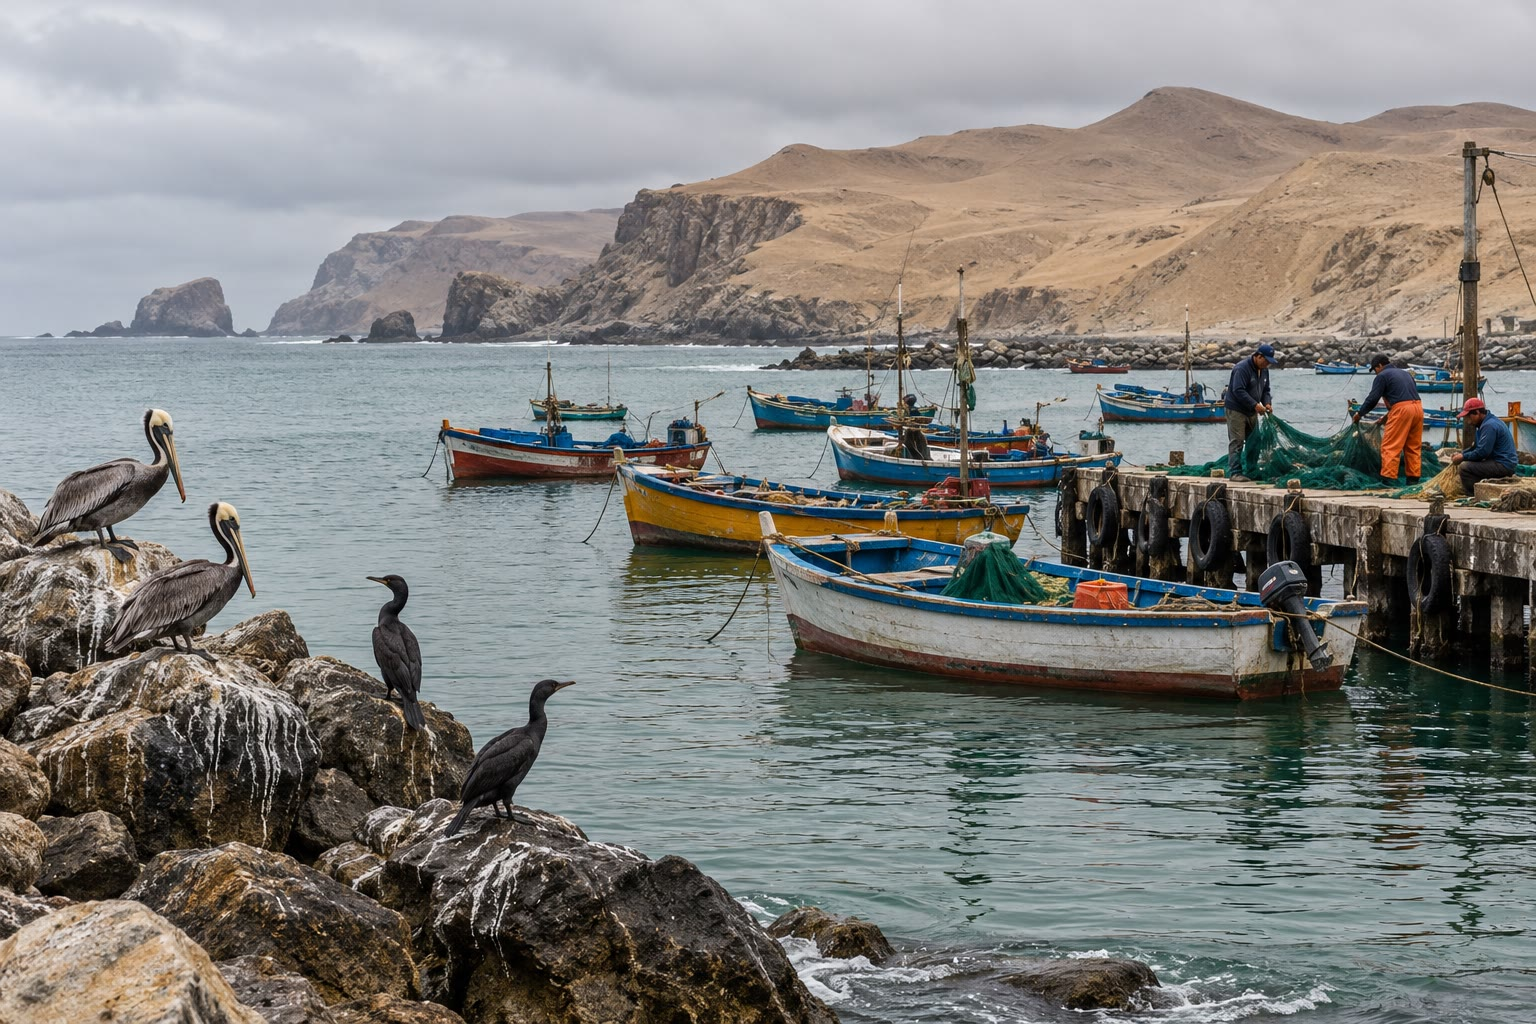
\includegraphics[width=\linewidth]{images/book4/ai/b2-fishing-harbour.jpg}

{\scriptsize Barcas de pesca en un puerto de una costa desértica con aguas frías de afloramiento
(ilustración generada por IA).}
\end{minipage}
% ledger: climategov:enso-history, cheung26:peru, stewart:upwelling
\end{history}

¿Por qué oscila el sistema? Porque el océano y la atmósfera del Pacífico ecuatorial
refuerzan cada uno las anomalías del otro.

\begin{definition}[Retroalimentación de Bjerknes]\label{def:b2:climate-variability:bjerknes}
La \emph{retroalimentación de Bjerknes}\index{retroalimentacion de Bjerknes@retroalimentación de Bjerknes} es la retroalimentación positiva entre la
temperatura de la superficie del mar, los vientos y las corrientes oceánicas del Pacífico ecuatorial: un calentamiento
del este debilita el contraste este--oeste de temperatura y presión, y por tanto los alisios;
unos alisios más débiles dejan que el agua cálida del oeste se extienda hacia el este y hacen subir menos agua fría en el
este, lo que calienta aún más el este. El mismo bucle amplifica un enfriamiento.
\end{definition}
% ledger: thirumalai24:bjerknes, cpc:enso-faq-timing

\begin{omfigure}
\centering
\begin{tikzpicture}[font=\small, >=Stealth, box/.style={draw, rounded corners=2pt, fill=omDef!8,
  align=center, text width=4.3cm, minimum height=1.05cm, inner sep=3pt}]
\node[box] (a) at (0,2) {Pacífico ecuatorial oriental\\más cálido de lo habitual};
\node[box] (b) at (6.2,2) {menor contraste este--oeste\\de temperatura y presión};
\node[box] (c) at (6.2,0) {alisios más débiles};
\node[box] (d) at (0,0) {el agua cálida avanza al este,\\sube menos agua fría};
\draw[->, very thick, ocRed] (a) -- (b);
\draw[->, very thick, ocRed] (b) -- (c);
\draw[->, very thick, ocRed] (c) -- (d);
\draw[->, very thick, ocRed] (d) -- (a);
\node[ocRed, font=\bfseries] at (3.1,1) {$+$};
\end{tikzpicture}
\par\smallskip{\small La \omterm{def:b2:climate-variability:bjerknes}{retroalimentación de Bjerknes}, dibujada para un calentamiento; con todas las flechas invertidas, el
mismo bucle acentúa un enfriamiento. Un bucle positivo de este tipo amplifica una pequeña perturbación.}
\end{omfigure}
% ledger: thirumalai24:bjerknes

Una retroalimentación positiva explica cómo crece una anomalía, no cómo empieza ni cómo termina. Según una explicación actual,
un El~Niño empieza cuando fluctuaciones aleatorias de los alisios debilitan las corrientes ecuatoriales que
retienen el agua cálida en el oeste; la piscina cálida se extiende hacia el este, la convección la sigue, la
\omterm{def:b2:climate-variability:bjerknes}{retroalimentación de Bjerknes} toma el relevo y el episodio crece. Los episodios de La~Niña, según la misma explicación,
los desencadena un El~Niño precedente. Los modelos más sencillos que hacen oscilar el sistema, entre ellos el oscilador
de recarga, acoplan dos magnitudes: la anomalía de temperatura de la superficie del mar del Pacífico
central y el volumen de agua cálida de la capa superior del océano almacenado a lo largo del ecuador. La anomalía de
temperatura vacía o rellena esa reserva a través de los vientos que impulsa, y la reserva, a través de la
profundidad de la termoclina, prepara la fase siguiente. El \cref{exo:b2:climate-variability:10} resuelve
un par de ecuaciones así.
% ledger: thirumalai24:bjerknes, stuecker25:ro

Para seguir el ENOS, los centros de vigilancia usan índices.

\begin{definition}[Índice Niño 3.4; Índice Oceánico de El Niño]\label{def:b2:climate-variability:oni}
El \emph{índice Niño 3.4}\index{indice Nino 3.4@índice Niño 3.4} es la anomalía mensual de la temperatura de la superficie del mar
promediada sobre la región \ang{5} N--\ang{5} S, \ang{170} W--\ang{120} W, respecto de
la \omterm{def:b2:climate-variability:modes}{climatología} de un periodo base de 30 años centrado en el año, actualizado cada cinco años. El
\emph{Índice Oceánico de El Niño}\index{Indice Oceanico de El Nino@Índice Oceánico de El Niño} (ONI) es su media móvil de tres meses. Un
episodio de El~Niño (de La~Niña) es una sucesión de al menos cinco trimestres consecutivos solapados
con el ONI igual o superior a \qty{+0.5}{\celsius} (igual o inferior a \qty{-0.5}{\celsius}).
\end{definition}
% ledger: cpc:oni-def, cpc:enso-faq

Los trimestres se solapan: DEF, EFM, FMA, etc., cada uno la media de tres meses, y cada uno comparte dos
meses con el siguiente. Un segundo índice, el Índice de \omterm{def:b2:climate-variability:enso}{Oscilación del Sur}, sigue la atmósfera: se
calcula a partir de las desviaciones de la diferencia de presión entre Tahití y Darwin, y es negativo
durante El~Niño y positivo durante La~Niña. Desde febrero de 2026 el índice oficial para vigilar el
ENOS es un ONI relativo, calculado a partir de la anomalía Niño 3.4 menos la anomalía media de todo el
océano tropical entre \ang{20} N y \ang{20} S, y reescalado después a la amplitud del ONI. Al estar
medido respecto del conjunto de los trópicos, depende menos de la elección del periodo base mientras los océanos
se calientan, y está mejor relacionado con la lluvia del Pacífico tropical. En septiembre de 2026 la
anomalía relativa de la región Niño 3.4 fue de \qty{2.08}{\celsius}, frente a los \qty{2.56}{\celsius}
del \cref{ex:b2:climate-variability:anomaly}: alrededor de medio grado de la anomalía tradicional era el
calor del conjunto de los océanos tropicales.
% ledger: cpc:enso-faq-so, pns:roni, data:b4-rnino34

\begin{omfigure}
\centering
% figdata/bachelor-2/climvar.py part oni
\begin{tikzpicture}
\begin{axis}[width=\linewidth, height=6.0cm, xmin=1950, xmax=2027, ymin=-2.4, ymax=3.0,
  xlabel={año}, ylabel={índice (\unit{\celsius})}, tick label style={font=\scriptsize},
  label style={font=\small}, xtick={1950,1960,...,2020}, x tick label style={/pgf/number
  format/1000 sep={}}, legend style={font=\scriptsize, at={(0.5,1.02)}, anchor=south,
  draw=none, legend columns=3, /tikz/every even column/.append style={column sep=6pt}},
  legend cell align=left]
\addplot[fill=ocRed!70, draw=none, area legend] table[x=t, y=pos]
  {figdata/out/bachelor-2-climvar-oni.dat} \closedcycle;
\addlegendentry{ONI, lado de El Niño}
\addplot[fill=ocBlue!70, draw=none, area legend] table[x=t, y=neg]
  {figdata/out/bachelor-2-climvar-oni.dat} \closedcycle;
\addlegendentry{ONI, lado de La Niña}
\addplot[black, thin] table[x=t, y=roni] {figdata/out/bachelor-2-climvar-oni.dat};
\addlegendentry{ONI relativo}
\addplot[black!60, densely dashed, domain=1950:2027, samples=2] {0.5};
\addplot[black!60, densely dashed, domain=1950:2027, samples=2] {-0.5};
\end{axis}
\end{tikzpicture}
\par\smallskip{\small El \omterm{def:b2:climate-variability:oni}{Índice Oceánico de El Niño} de DEF 1950 a JAS 2026 (un valor por
trimestre, representado en su mes central), y el ONI relativo, índice oficial desde
febrero de 2026; en trazos, los umbrales $\pm\qty{0.5}{\celsius}$. Datos: NOAA Climate Prediction
Center, descargados el 23 de octubre de 2026.}
\end{omfigure}
% ledger: data:b4-oni, data:b4-roni

Contados con la regla de los cinco trimestres sobre la tabla del Climate Prediction Center, el ONI muestra 25
episodios de El~Niño y 21 de La~Niña entre 1950 y el verano de 2026. Los máximos más fuertes de El~Niño
fueron de \qty{2.4}{\celsius} a finales de 1997 y de \qty{2.6}{\celsius} a finales de 2015. Los dos índices
divergen sobre todo en los últimos años: en julio--septiembre de 2026 el ONI estaba en \qty{2.2}{\celsius} y
el índice relativo en \qty{1.7}{\celsius}.
% ledger: data:b4-oni, data:b4-roni

\begin{dated}{2026}
En su discusión del 8 de octubre de 2026, el Climate Prediction Center mantuvo su aviso de El~Niño: la
anomalía relativa Niño 3.4 había alcanzado \qty{+2.1}{\celsius} en septiembre, partes del Pacífico ecuatorial
oriental estaban más de \qty{4}{\celsius} por encima de la media, el agua en profundidad en el este
más de \qty{10}{\celsius} por encima, y los índices de la \omterm{def:b2:climate-variability:enso}{Oscilación del Sur} eran claramente
negativos. Se juzgaba probable un
El~Niño de fuerte a muy fuerte hasta enero--marzo de 2027, y la probabilidad de que
el índice relativo superara \qty{2.5}{\celsius}, por encima de todos los episodios desde 1950, se cifraba en un
\qty{83}{\percent} para octubre--diciembre.
% ledger: cpc:edd-2026-10, data:b4-rnino34
\end{dated}

\section{La Oscilación del Atlántico Norte y las teleconexiones}\label{sec:b2:climate-variability:nao}

\begin{definition}[Oscilación del Atlántico Norte]\label{def:b2:climate-variability:nao}
La \emph{Oscilación del Atlántico Norte}\index{Oscilacion del Atlantico Norte@Oscilación del Atlántico Norte} (NAO) es el modo dominante
de la variabilidad atmosférica sobre el Atlántico Norte: un balancín de presión al nivel del mar entre la
baja de Islandia y el anticiclón de las Azores. Su índice es positivo cuando ambos son más intensos que la media, de modo
que la diferencia de presión entre ellos es grande, y negativo cuando ambos son más débiles.
\end{definition}
% ledger: ipccgl:other-modes, climategov:nao, cpc:nao-teledoc

La NAO gobierna los vientos del oeste del capítulo anterior. En su fase positiva, la mayor diferencia
de presión impulsa una corriente en chorro atlántica más fuerte y desplaza al norte la trayectoria de las borrascas: el norte de Europa
tiene un invierno más tormentoso, más húmedo y más suave, el sur de Europa uno más seco, el este de América del Norte
menos irrupciones de aire frío, y Groenlandia un invierno más frío. La fase negativa invierte estas
anomalías. A finales del siglo XVIII un misionero ya observó que los inviernos suaves en
Groenlandia coincidían con inviernos duros en Dinamarca, y a la inversa.
% ledger: climategov:nao, cpc:nao-teledoc

La NAO es una de las configuraciones más destacadas de la atmósfera en todas las estaciones, y está
fuertemente correlacionada con otro modo, la Oscilación Ártica. También varía a lo largo de décadas: la fase negativa dominó
desde mediados de la década de 1950 hasta el invierno de 1978--79, y la fase positiva de 1979--80 a 1994--95.
% ledger: cpc:nao-teledoc, climategov:nao

\begin{omfigure}
\centering
% figdata/bachelor-2/climvar.py part nao
\begin{tikzpicture}
\begin{axis}[width=\linewidth, height=5.4cm, xmin=1950, xmax=2027, ymin=-1.9, ymax=1.9,
  ytick={-1,0,1},
  xlabel={invierno (año de su enero)}, ylabel={índice NAO (media DEF)},
  tick label style={font=\scriptsize}, label style={font=\small}, xtick={1950,1960,...,2020},
  x tick label style={/pgf/number format/1000 sep={}}, legend style={font=\scriptsize,
  at={(0.5,1.02)}, anchor=south, draw=none, legend columns=2,
  /tikz/every even column/.append style={column sep=6pt}},
  legend cell align=left, unbounded coords=jump]
\addplot[ybar, bar width=0.6, fill=omDef!55, draw=none, area legend] table[x=year, y=nao]
  {figdata/out/bachelor-2-climvar-nao.dat};
\addlegendentry{media invernal}
\addplot[ocRed, thick] table[x=year, y=run5] {figdata/out/bachelor-2-climvar-nao.dat};
\addlegendentry{media móvil de 5 inviernos}
\end{axis}
\end{tikzpicture}
\par\smallskip{\small La media invernal (diciembre--febrero) del índice NAO mensual del NOAA
Climate Prediction Center, 1951--2026, en desviaciones típicas, con su media móvil centrada de cinco
inviernos. El invierno más bajo es 2010 ($-1.67$), el más alto 2015 ($+1.66$).}
\end{omfigure}
% ledger: data:b4-nao, cpc:nao-teledoc

La NAO, el ENOS y los demás modos actúan lejos de donde se miden.

\begin{definition}[Teleconexión]\label{def:b2:climate-variability:teleconnection}
Una \emph{teleconexión}\index{teleconexion@teleconexión} es una asociación entre variables climáticas en
lugares fijos muy alejados, enlazados por procesos físicos a lo largo de caminos en la atmósfera o el
océano, como trenes de \omterm{def:b2:weather-systems:rossby}{ondas de Rossby}, desplazamientos de la corriente en chorro y de las trayectorias de las borrascas, o cambios
de la circulación de Walker.
\end{definition}
% ledger: ipccgl:teleconnection

Durante El~Niño la lluvia de los trópicos cambia desde Indonesia hasta América del Sur, aproximadamente media vuelta
al mundo, y desde los trópicos las anomalías viajan a las latitudes medias por los caminos
de la definición; el \omterm{def:b2:climate-variability:monsoon}{monzón} indio de la sección anterior es uno de sus extremos. Se han nombrado otros modos
en cada océano: el dipolo del océano Índico, un balancín este--oeste de la temperatura de la superficie
del mar en el océano Índico tropical cuya fase positiva enfría el mar frente a Sumatra y Java
y lo calienta frente a Somalia, que se desarrolla en el verano boreal, madura en otoño y cambia
la lluvia de Australia, el Sudeste Asiático y África oriental; el modo anular del sur, los cambios de
intensidad y de latitud del cinturón de vientos del oeste alrededor de la Antártida; y la variabilidad decenal del
Pacífico, más lenta que el ENOS.
% ledger: cpc:enso-faq, ipccgl:other-modes, ipccgl:teleconnection, narang24:enso-monsoon

\section{El océano como memoria}\label{sec:b2:climate-variability:memory}

El \cref{ch:b2:weather-systems} halló que la atmósfera olvida su tiempo en unas dos semanas.
Una anomalía climática que dura una estación tiene que almacenarse en algún sitio, y el depósito evidente es la capa
de mezcla del océano: una capa de mezcla más profunda contiene más calor y tiene más inercia térmica. El modelo más sencillo trata la
anomalía como un depósito que pierde calor hacia la atmósfera.
% ledger: shi22:memory

\begin{proposition}[Tiempo de amortiguamiento de una anomalía de la capa de mezcla]\label{prop:b2:climate-variability:damping}
Sea una capa de mezcla de espesor $h$, densidad $\rho$ y calor específico $c_p$ que lleva una anomalía de temperatura
$T'$, y sea que la superficie pierde hacia la atmósfera un flujo de calor adicional $\alpha T'$ por unidad de área,
con $\alpha > 0$. Entonces, sin otro forzamiento,
\[
  T'(t) = T'(0)\,\mathrm{e}^{-t/\tau}, \qquad \tau = \frac{\rho\,c_p\,h}{\alpha} .
\]
\end{proposition}

\begin{proof}
El contenido de calor de la anomalía por unidad de área es $\rho c_p h T'$; el primer principio da $\rho c_p h
\,\mathrm{d}T'/\mathrm{d}t = -\alpha T'$, una ecuación lineal cuya solución es el decaimiento exponencial
con la constante de tiempo $\tau$.
\end{proof}
% ledger: shi22:memory

\begin{example}[La memoria de un océano de latitudes medias]\label{ex:b2:climate-variability:tau}
Sobre los océanos de las latitudes medias, el flujo de calor en superficie responde a una anomalía de temperatura de la
superficie del mar con un valor medio $\alpha = \qty{16.1}{W.m^{-2}.K^{-1}}$. Para una capa de mezcla
de \qty{50}{m} de espesor, con $\rho = \qty{1025}{kg/m^3}$ y $c_p = \qty{3992}{J.kg^{-1}.K^{-1}}$,
$\tau = 1025 \times 3992 \times 50/16.1 = \qty{1.27e7}{s} = \qty{147}{\day}$, casi cinco
meses; una capa de \qty{100}{m} recuerda el doble de tiempo.
\end{example}
% ledger: wang24:shff, noaa:seawater-1025, teos10:cp0

Las anomalías reales están además forzadas, cada día, por el tiempo: flujos de calor aleatorios que, por sí solos,
darían un ruido blanco, sin memoria de un mes al siguiente. Añadidos al amortiguamiento, dan
la ecuación $\mathrm{d}T'/\mathrm{d}t = -T'/\tau + F(t)$ con un $F$ aleatorio: el océano suma
el forzamiento aleatorio durante un tiempo del orden de $\tau$ y lo olvida más allá. El resultado se llama
ruido rojo. Su correlación con desfase, la correlación entre la anomalía y ella misma algún tiempo después,
cae como $\mathrm{e}^{-\text{desfase}/\tau}$ (se admite), y las variaciones lentas son en él mucho más intensas
que en el forzamiento. Este modelo estocástico de la memoria del océano es la referencia estándar
con la que se mide la persistencia de las anomalías reales, una fuente de predictibilidad más allá de
las escalas de tiempo del tiempo meteorológico; como el espesor de la capa de mezcla fija la memoria, la reducción del espesor de las
capas de mezcla proyectada para este siglo implica una memoria más corta.
% ledger: shi22:memory

\begin{omfigure}
\centering
% figdata/bachelor-2/climvar.py parts rednoise, acf
\begin{tikzpicture}
\begin{groupplot}[group style={group size=2 by 1, horizontal sep=1.6cm},
  tick label style={font=\scriptsize}, label style={font=\small}]
\nextgroupplot[width=0.62\linewidth, height=5.0cm, xmin=0, xmax=360, ymin=-1.6, ymax=1.6,
  xlabel={mes}, ylabel={anomalía (\unit{K})}, xtick={0,60,...,360},
  legend style={font=\scriptsize, at={(0.5,1.02)}, anchor=south, draw=none, legend columns=2},
  legend cell align=left]
\addplot[black!45, thin] table[x=month, y=white] {figdata/out/bachelor-2-climvar-rednoise.dat};
\addlegendentry{ruido blanco}
\addplot[ocRed, thick] table[x=month, y=red] {figdata/out/bachelor-2-climvar-rednoise.dat};
\addlegendentry{ruido rojo, $\tau = \qty{147}{\day}$}
\nextgroupplot[width=0.36\linewidth, height=5.0cm, xmin=0, xmax=24, ymin=0, ymax=1.05,
  xlabel={desfase (meses)}, ylabel={correlación con desfase}, xtick={0,6,...,24},
  legend style={font=\scriptsize, at={(0.98,0.98)}, anchor=north east, draw=none},
  legend cell align=left]
\addplot[black, densely dashed] table[x=lag_months, y=theory] {figdata/out/bachelor-2-climvar-acf.dat};
\addlegendentry{$\mathrm{e}^{-\text{desfase}/\tau}$}
\addplot[only marks, mark=*, mark size=1.1pt, ocRed] table[x=lag_months, y=sample]
  {figdata/out/bachelor-2-climvar-acf.dat};
\addlegendentry{simulada}
\end{groupplot}
\end{tikzpicture}
\par\smallskip{\small Un ruido rojo y un ruido blanco de la misma desviación típica, 0.5~K, en forma de
medias mensuales a lo largo de 30 años (izquierda): la capa de mezcla del
\cref{ex:b2:climate-variability:tau} convierte un forzamiento diario aleatorio en oscilaciones lentas. Derecha: la correlación
con desfase de una simulación de 2000 años frente a $\mathrm{e}^{-\text{desfase}/\tau}$.}
\end{omfigure}
% ledger: shi22:memory, wang24:shff

El ENOS necesita algo más que esta memoria pasiva. Sus anomalías afectan no solo a la capa de mezcla, sino a
toda la capa cálida por encima de la termoclina, que se desplaza decenas de metros, y los vientos que
impulsan las anomalías actúan de nuevo sobre el océano a través del bucle de Bjerknes. El océano aporta la lentitud,
la atmósfera el acoplamiento; ninguno de los dos por sí solo produce la oscilación. Esa lentitud es lo que tuvieron en cuenta los
predictores de octubre de 2026 cuando juzgaron probable que un El~Niño fuerte durara hasta
enero--marzo de 2027.
% ledger: cpc:enso-faq-features, cpc:enso-faq-timing, climategov:enso-history, cpc:edd-2026-10

\section*{Ejercicios}\label{sec:b2:climate-variability:exercises}

Datos de los ejercicios, salvo aviso contrario: agua de mar $\rho = \qty{1025}{kg/m^3}$ y $c_p =
\qty{3992}{J.kg^{-1}.K^{-1}}$; aire $c_p = \qty{1004.5}{J.kg^{-1}.K^{-1}}$; $g =
\qty{9.81}{m.s^{-2}}$; el coeficiente de amortiguamiento del flujo de calor en superficie $\alpha =
\qty{16.1}{W.m^{-2}.K^{-1}}$; un mes son $365.25/12 = 30.44$ días.
% ledger: noaa:seawater-1025, teos10:cp0, wang24:shff

\begin{exercise}[$\star$]\label{exo:b2:climate-variability:1}
En la región Niño 3.4 la temperatura media de la superficie del mar fue de \qty{29.27}{\celsius} en septiembre
de 2026 y de \qty{28.79}{\celsius} en septiembre de 1997; las \omterm{def:b2:climate-variability:modes}{climatologías} usadas para esos dos septiembres
fueron \qty{26.71}{\celsius} y \qty{26.73}{\celsius}. (a) Calcúlense las dos anomalías. (b) ¿Qué
septiembre fue más cálido, y qué anomalía mayor? (c) ¿Por qué la \omterm{def:b2:climate-variability:modes}{climatología} no es la misma para los
dos años?
\end{exercise}
% ledger: data:b4-nino34, cpc:oni-def

\begin{exercise}[$\star$]\label{exo:b2:climate-variability:2}
Las anomalías mensuales Niño 3.4 de junio a diciembre de 2023 fueron 0.79, 0.95, 1.28, 1.55, 1.68, 2.01
y \qty{2.02}{\celsius}. (a) Calcúlese el ONI de los trimestres JJA a OND. (b) La tabla del
Climate Prediction Center da 1.0, 1.3, 1.5, 1.7 y 1.9. Compárese. (c) ¿En qué trimestre alcanzó el
ONI por primera vez el umbral de un episodio fuerte, \qty{1.5}{\celsius}?
\end{exercise}
% ledger: data:b4-nino34-2023, data:b4-oni-cases

\begin{exercise}[$\star$]\label{exo:b2:climate-variability:3}
En un mes dado, la presión en superficie está por encima de la media en Darwin y por debajo de la media en Tahití.
(a) ¿Cuál es el signo del Índice de \omterm{def:b2:climate-variability:enso}{Oscilación del Sur}? (b) ¿Qué fase del ENOS sugiere?
(c) ¿Qué cabe esperar de los alisios sobre el Pacífico ecuatorial oriental, y de la
lluvia sobre Indonesia?
\end{exercise}
% ledger: cpc:enso-faq-so, cpc:enso-faq-features

\begin{exercise}[$\star$]\label{exo:b2:climate-variability:4}
(a) La lluvia de junio a septiembre de 2018 sobre la India fue de \qty{804.1}{mm}, frente a una
media del largo periodo de \qty{880.6}{mm}. Exprésese como porcentaje de la media y clasifíquese
la estación. (b) En la costa de Kerala las medias de junio, julio, agosto y septiembre son 556,
659, 427 y \qty{252}{mm}. ¿Qué fracción de la lluvia de la estación cae en julio?
\end{exercise}
% ledger: imd:lpa

\begin{exercise}[$\star\star$]\label{exo:b2:climate-variability:5}
(a) Calcúlese el tiempo de amortiguamiento de una anomalía en capas de mezcla de \qty{50}{m} y \qty{100}{m} de espesor.
(b) Calcúlese, para cada una, la correlación con desfase de la anomalía al cabo de un mes. (c) Los modelos climáticos
proyectan capas de mezcla menos profundas en un clima más cálido. ¿Qué efecto tiene eso sobre la memoria del
océano?
\end{exercise}
% ledger: wang24:shff, shi22:memory

\begin{exercise}[$\star\star$]\label{exo:b2:climate-variability:6}
Se observa una anomalía de temperatura de la superficie del mar de \qty{+1.2}{K} sobre una capa de mezcla de \qty{50}{m}
de espesor. (a) Sin más forzamiento, ¿qué anomalía queda al cabo de tres meses, y al cabo de seis? (b)
Una predicción así, que se limita a dejar decaer la anomalía presente, se llama predicción de persistencia.
¿Por qué es mejor que suponer que no hay anomalía, y por qué empeora con el tiempo?
\end{exercise}

\begin{exercise}[$\star\star$]\label{exo:b2:climate-variability:7}
En junio el suelo de los desiertos del noroeste de la India y de Pakistán envía unos
\qty{160}{W/m^2} de calor al aire. (a) ¿Cuánta energía es eso por metro cuadrado y por día?
(b) Si todo se quedara en la capa comprendida entre el suelo a \qty{1000}{hPa} y \qty{850}{hPa}, ¿a qué
ritmo se calentaría esa capa? (c) En realidad la baja térmica no se calienta a ese ritmo semana tras semana.
Nómbrense dos maneras en que el calor puede salir de la capa.
\end{exercise}
% ledger: imd:heat-low

\begin{exercise}[$\star\star$]\label{exo:b2:climate-variability:8}
El índice NAO mensual fue de $-1.93$ en diciembre de 2009, $-1.11$ en enero de 2010 y $-1.98$ en
febrero de 2010. (a) Calcúlese la media invernal. (b) En 1951--2026 las medias invernales van de
$-1.67$ a $+1.66$. Sitúese este invierno. (c) ¿Qué tiempo invernal cabría esperar en el norte de
Europa, en el sur de Europa y en el este de Estados Unidos?
\end{exercise}
% ledger: data:b4-nao, climategov:nao

\begin{exercise}[$\star\star$]\label{exo:b2:climate-variability:9}
Una región pertenece al dominio monzónico global cuando la lluvia media de su verano local supera a la
de su invierno en más de \qty{2.5}{mm} al día. (a) Una estación inventada del hemisferio
norte recibe en promedio \qty{9.3}{mm} al día en junio--agosto y \qty{0.4}{mm} al día en
diciembre--febrero. ¿Está en el dominio? (b) Una estación inventada del hemisferio sur
recibe \qty{4.2}{mm} al día en junio--agosto y \qty{6.1}{mm} al día en diciembre--febrero. ¿Lo
está? (c) En la costa de Kerala, la lluvia media de junio a septiembre (122 días) es de 556, 659, 427 y
\qty{252}{mm} mes a mes. Calcúlese su intensidad diaria media, y la intensidad invernal por encima de la cual Kerala,
tomando junio--septiembre como su verano, quedaría fuera del dominio. (d) ¿Por qué el criterio
usa la diferencia entre las estaciones y no la lluvia total del año?
\end{exercise}
% ledger: ipccgl:monsoon, imd:lpa

\begin{exercise}[$\star\star\star$]\label{exo:b2:climate-variability:10}
Un oscilador de recarga sencillo escribe la anomalía de temperatura Niño 3.4 $T$ y la anomalía $H$ del
agua cálida almacenada a lo largo del ecuador como $\dot T = aH$, $\dot H = -bT$, con $a, b > 0$. (a) Demuéstrese
que $T$ oscila, con el periodo $2\pi/\sqrt{ab}$. (b) ¿Qué producto $ab$ da un periodo de
cuatro años? (c) Con amortiguamiento, $\dot T = aH - rT$ y $\dot H = -bT - rH$, demuéstrese que
$(T\,\mathrm{e}^{rt}, H\,\mathrm{e}^{rt})$ cumple las ecuaciones sin amortiguamiento. Con $r = 0.25$ por
año, ¿en qué factor disminuye la amplitud en un periodo? (d) ¿Qué debe mantener la oscilación
real?
\end{exercise}
% ledger: stuecker25:ro, thirumalai24:bjerknes, ipccgl:enso

\begin{exercise}[$\star\star\star$]\label{exo:b2:climate-variability:11}
La región Niño 3.4 se extiende \ang{10} en latitud y \ang{50} en longitud a lo largo del ecuador
(tómese un radio terrestre de \qty{6371}{km}). (a) Calcúlese su área. (b) ¿Cuánto calor hace falta para
calentar \qty{2}{K} una capa de \qty{100}{m} de espesor sobre esa área? (c) ¿Qué flujo de calor adicional en superficie,
mantenido durante seis meses, lo aportaría? (d) Durante El~Niño los alisios se debilitan y la
termoclina del este se hunde. ¿De dónde más puede venir el calor?
\end{exercise}
% ledger: cpc:oni-def, cpc:enso-faq-features

\begin{exercise}[$\star\star\star$]\label{exo:b2:climate-variability:12}
Trátese la \omterm{def:b2:climate-variability:bjerknes}{retroalimentación de Bjerknes} como un bucle que devuelve, como calentamiento adicional, una fracción $g$ de todo
calentamiento que pasa por él. (a) Una ráfaga de viento del oeste calienta el este \qty{0.3}{K}. Demuéstrese
que el calentamiento total es $0.3/(1 - g)$, y calcúlese para $g = 0.5$, 0.8 y 0.9. (b) ¿Qué
ocurre si $g \geq 1$, y qué debe entonces limitar el episodio? (c) ¿Por qué $g$ debería ser máximo en la
estación en que el Pacífico ecuatorial está más cálido?
\end{exercise}
% ledger: thirumalai24:bjerknes, cpc:enso-faq-timing

\begin{problem}[{Problema de fin de semana --- Contar los El Niño}]\label{pb:b2:climate-variability:1}
De las temperaturas mensuales del mar al registro de El~Niño desde 1950, y al océano que lo hace
posible. Úsense los datos de los ejercicios.

\medskip\noindent\textbf{Parte I --- De los meses a los trimestres.}
Las anomalías mensuales Niño 3.4 de abril de 1997 a enero de 1998 fueron 0.26, 0.75, 1.13, 1.52, 1.80,
2.06, 2.26, 2.42, 2.36 y \qty{2.33}{\celsius}.
\begin{enumerate}
  \item Calcúlese el ONI del trimestre AMJ 1997.
  \item Calcúlese el ONI de MJJ, JJA y JAS.
  \item Calcúlese el ONI de ASO, SON, OND y NDE.
  \item La tabla del Climate Prediction Center da 0.7, 1.1, 1.5, 1.8, 2.0, 2.2, 2.3 y
        2.4 para estos ocho trimestres. Compárese.
  \item ¿Por qué el índice promedia tres meses en lugar de usar meses sueltos?
  \item ¿En qué trimestre se volvió fuerte el episodio de 1997 ($\geq \qty{1.5}{\celsius}$), y en
        qué valor culminó?
\end{enumerate}

\medskip\noindent\textbf{Parte II --- La regla de los cinco trimestres.}
El ONI del Climate Prediction Center para 2018 a 2020 dice, trimestre a trimestre de DEF a
NDE: 2018: $-0.7$, $-0.7$, $-0.5$, $-0.3$, $-0.1$, 0.1, 0.2, 0.3, 0.5, 0.8, 1.0, 1.1; 2019: 1.0,
0.9, 0.9, 0.8, 0.7, 0.6, 0.4, 0.2, 0.3, 0.5, 0.7, 0.8; 2020: 0.7, 0.7, 0.6, 0.3, 0.0, $-0.2$,
$-0.3$, $-0.4$, $-0.8$, $-1.0$, $-1.1$, $-1.1$; después DEF 2021 $-1.0$ y EFM 2021 $-0.9$. El
ONI relativo dice, desde SON 2018: 0.62, 0.82, 0.78; 2019: 0.68, 0.64, 0.57, 0.53, 0.37, 0.24,
0.04, $-0.12$, $-0.01$, 0.15, 0.29, 0.22; 2020: 0.14, 0.10, 0.02, $-0.25$, $-0.55$, $-0.72$,
$-0.76$, $-0.85$, $-1.16$, $-1.37$, $-1.46$, $-1.39$.
\begin{enumerate}[resume]
  \item Hállense los episodios de El~Niño de 2018--2020 según el ONI: primer y último trimestre de cada uno.
  \item ¿Cuántos trimestres dura cada uno?
  \item ¿En qué trimestre empieza la siguiente La~Niña según el ONI, y por qué hacen falta los
        valores de 2021 para estar seguro de ello?
  \item Hállense los episodios de El~Niño según el ONI relativo, y el primer trimestre de La~Niña.
  \item ¿Es el episodio de finales de 2019 un El~Niño según el ONI relativo? Explíquese la diferencia
        entre los dos índices en 2019.
\end{enumerate}

\medskip\noindent\textbf{Parte III --- Los El Niño fuertes.}
Los episodios de El~Niño desde 1950 cuyo ONI máximo alcanzó al menos \qty{1.5}{\celsius} empezaron en los
trimestres MAM 1957, AMJ 1965, AMJ 1972, AMJ 1982, JAS 1986, AMJ 1991, AMJ 1997, JJA 2009, SON 2014,
AMJ 2023 y MAM 2026, con máximos de 1.7, 1.8, 1.8, 2.1, 1.5, 1.5, 2.4, 1.5, 2.6, 2.0 y, en
JAS 2026, \qty{2.2}{\celsius} y en aumento. Cuéntese en años, a partir del año en que empezó cada uno.
\begin{enumerate}[resume]
  \item ¿Cuántos episodios fuertes hay?
  \item Enumérense los intervalos entre los inicios de episodios fuertes sucesivos.
  \item ¿Qué intervalo es el más corto, y cuál el más largo?
  \item Calcúlese el intervalo medio de dos maneras: como la media de los intervalos, y como el tiempo
        desde el primer inicio hasta el último dividido por el número de intervalos. ¿Por qué coinciden?
  \item El episodio de 2026 seguía creciendo cuando terminan los datos. ¿Por qué cuenta, sin embargo,
        como episodio fuerte, y por qué ningún dato posterior puede cambiar su inicio?
  \item Las preguntas frecuentes del Climate Prediction Center dicen que El~Niño y La~Niña se producen cada 3 a 5
        años. ¿Es coherente con eso el intervalo medio de los episodios fuertes?
\end{enumerate}

\medskip\noindent\textbf{Parte IV --- Por qué el ENOS necesita el océano.}
Tómense una capa de mezcla de \qty{50}{m} de espesor y una columna de aire de \qty{1000}{hPa}.
\begin{enumerate}[resume]
  \item Calcúlese el tiempo de amortiguamiento de una anomalía de la capa de mezcla.
  \item Calcúlese la capacidad calorífica por metro cuadrado de la capa de mezcla y de toda la columna
        de aire que hay encima.
  \item ¿Qué espesor de agua de mar tiene la capacidad calorífica de toda la atmósfera que hay encima?
  \item Calcúlese el tiempo de amortiguamiento de una anomalía llevada solo por la columna de aire, con el mismo
        $\alpha$.
  \item ¿Por qué el océano puede llevar una anomalía del ENOS de una estación a la siguiente, y la
        atmósfera no?
  \item En resumen: ¿cuántos años, en promedio, separan los inicios de episodios fuertes sucesivos de El~Niño
        desde 1950?
\end{enumerate}
\end{problem}
% ledger: data:b4-nino34, data:b4-oni, data:b4-oni-cases, data:b4-roni-cases, cpc:enso-faq-timing, wang24:shff
